
%(BEGIN_QUESTION)
% Copyright 2011, Tony R. Kuphaldt, released under the Creative Commons Attribution License (v 1.0)
% This means you may do almost anything with this work of mine, so long as you give me proper credit

Væskenivået i scrubber (beholder V-5) reguleres av en Emerson DeltaV DCS, men noe er galt. Operatøren rapporterer 90\% nivå i LG-31 siktglass, mens settpunkt i DeltaV Operate er 75\%:

$$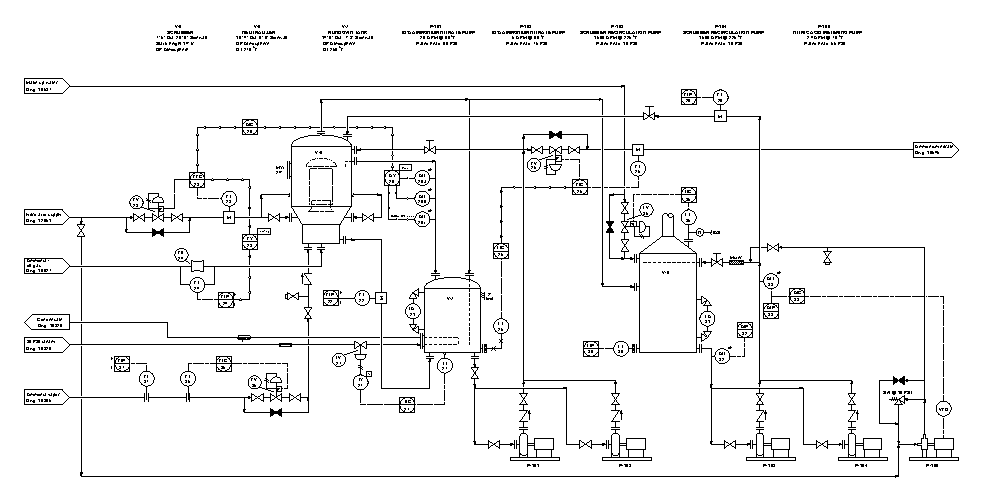
\includegraphics[width=15.5cm]{i0008rx01.eps}$$

\filbreak

I {\it DeltaV Control Studio} kan man vise ``online''-data i sanntid mellom funksjonsblokker. Ved online visning av denne sløyfen ser du følgende:

$$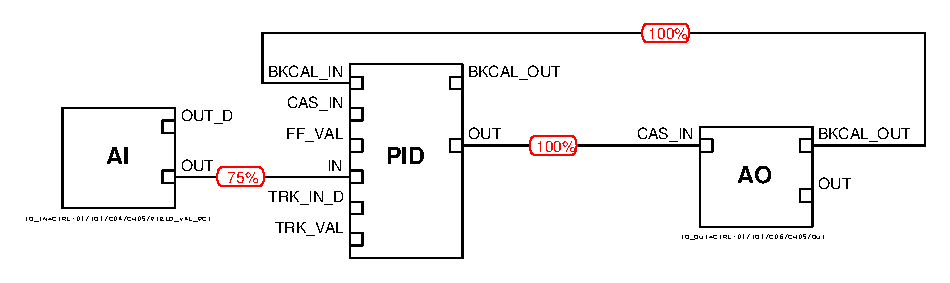
\includegraphics[width=15.5cm]{i00961x02.eps}$$

Vurder sannsynligheten for hver angitt feil basert på online-visningen. Se på én feil om gangen (ingen samtidige feil), og avgjør om feilen alene kan forklare {\it alle} målinger og symptomer.

% No blank lines allowed between lines of an \halign structure!
% I use comments (%) instead, so that TeX doesn't choke.

$$\vbox{\offinterlineskip
\halign{\strut
\vrule \quad\hfil # \ \hfil & 
\vrule \quad\hfil # \ \hfil & 
\vrule \quad\hfil # \ \hfil \vrule \cr
\noalign{\hrule}
%
% First row
{\bf Feil} & {\bf Mulig} & {\bf Umulig} \cr
%
\noalign{\hrule}
%
% Another row
Dårlig tuning i PID-funksjonsblokk &  &  \cr
%
\noalign{\hrule}
%
% Another row
LT-35 feilkalibrert, viser for lavt &  &  \cr
%
\noalign{\hrule}
%
% Another row
LT-35 feilkalibrert, viser for høyt &  &  \cr
%
\noalign{\hrule}
%
% Another row
Etterfyllingsvann avstengt &  &  \cr
%
\noalign{\hrule}
%
% Another row
Pumpe P-103 feilet (pumper ikke) &  &  \cr
%
\noalign{\hrule}
%
% Another row
Blokkventil på LG-31 siktglass tett &  &  \cr
%
\noalign{\hrule}
%
% Another row
Pumpe P-105 feilet (pumper ikke) &  &  \cr
%
\noalign{\hrule}
%
% Another row
Operatørfeil &  &  \cr
%
\noalign{\hrule}
} % End of \halign 
}$$ % End of \vbox


\underbar{file i00961}
%(END_QUESTION)





%(BEGIN_ANSWER)


%(END_ANSWER)





%(BEGIN_NOTES)

% No blank lines allowed between lines of an \halign structure!
% I use comments (%) instead, so that TeX doesn't choke.

$$\vbox{\offinterlineskip
\halign{\strut
\vrule \quad\hfil # \ \hfil & 
\vrule \quad\hfil # \ \hfil & 
\vrule \quad\hfil # \ \hfil \vrule \cr
\noalign{\hrule}
%
% First row
{\bf Feil} & {\bf Mulig} & {\bf Umulig} \cr
%
\noalign{\hrule}
%
% Another row
Dårlig tuning i PID-funksjonsblokk &  & $\surd$ \cr
%
\noalign{\hrule}
%
% Another row
LT-35 feilkalibrert, viser for lavt & $\surd$ &  \cr
%
\noalign{\hrule}
%
% Another row
LT-35 feilkalibrert, viser for høyt &  & $\surd$ \cr
%
\noalign{\hrule}
%
% Another row
Etterfyllingsvann avstengt &  & $\surd$ \cr
%
\noalign{\hrule}
%
% Another row
Pumpe P-103 feilet (pumper ikke) &  & $\surd$ \cr
%
\noalign{\hrule}
%
% Another row
Blokkventil på LG-31 siktglass tett & $\surd$ &  \cr
%
\noalign{\hrule}
%
% Another row
Pumpe P-105 feilet (pumper ikke) &  & $\surd$ \cr
%
\noalign{\hrule}
%
% Another row
Operatørfeil & $\surd$ &  \cr
%
\noalign{\hrule}
} % End of \halign 
}$$ % End of \vbox

Høy mettet regulatorutgang gjør transmitterkalibreringsfeil mest sannsynlig. Feil i siktglassavlesning kan være mulig, men forklarer ikke alene hvorfor regulatorutgangen er så høy.

%INDEX% DCS, programming: function block program
%INDEX% Process: ammonium nitrate production (realistic P&ID shown)
%INDEX% Process troubleshooting: diagnosing problem via online function block display in DCS

%(END_NOTES)

